\documentclass[10pt,a4paper]{article}
\usepackage[a4paper, top=2cm, bottom=1.5cm, left=1.5cm, right=1.5cm]{geometry} % Задать размеры полей.
\usepackage[warn]{mathtext} % Русские символы в формулах. Нужно писать до пакета babel. Указывает, что в формулах используются символы кириллицы, которые по умолчанию печатаются прямым шрифтом.
\usepackage[T2A]{fontenc}
\usepackage[utf8]{inputenc}
\usepackage[russian]{babel}
\usepackage{amsmath}
\usepackage{amssymb}
\usepackage{graphicx}
%\usepackage{floatrow}
\usepackage{booktabs}
\usepackage{wrapfig}
\usepackage{fancyhdr}
\usepackage{multicol}
\usepackage{xcolor}

\usepackage{float}
\usepackage{multirow}

\usepackage{subfigure}

% Объявляем новую команду для переноса строки внутри ячейки таблицы
\newcommand{\specialcell}[2][c]{%
	\begin{tabular}[#1]{@{}c@{}}#2\end{tabular}}

\newcommand{\figref}[1]{(См. рис. \ref{#1})}
\newcommand{\secref}[1]{(См. раздел. \ref{#1})}

\newcommand{\angstrom}{\text{\normalfont\AA}}
\newcommand{\e}[1]{\text{$\cdot10^{#1}$}}
\newcommand{\m}{\; м}
\newcommand{\mm}{\; мм}
\newcommand{\um}{\; мкм}
\newcommand{\A}{\; А}
\newcommand{\V}{\; В}
\newcommand{\uV}{\; мкВ}
\newcommand{\cels}{\; ^\circ С}

\pagestyle{fancy}
\fancyhead{}
\fancyhead[L]{\small Дедков Д.А., Маслов А.С., Изучение рассеяния медленных электронов на атомах. Эффект Рамзауэра. МФТИ, 2023 г.}
\fancyhead[R]{}
\fancyfoot[C]{\thepage}

\renewcommand{\cot}{\text{ctg}}

\author{\normalsize Дедков Денис, Маслов Артём \\
	\normalsize группа Б01-108а \\
	\normalsize 27.11.2023}
\date{}

\title{
	\Large Изучение рассеяния медленных электронов на атомах. Эффект Рамзауэра. \\ 
}

\begin{document}
\maketitle
	
	\subsection*{Цель и задачи работы:}
	\begin{enumerate}
		\item Исследовать энергетические зависимости вероятности рассеяния электронов атомами инертного газа. 
		
		\item Определить энергии электронов, при которых наблюдается просветление инертного газа.
		
		\item Оценить размер внешней электронной оболочки инертного газа.
		
		\item По значению измеренного ионизационного потенциала определяется, каким газом заполнен тиратрон.
	\end{enumerate}
	
	\subsection*{Описание экспериментальной установки}
	
	\begin{figure}[H]
		\centering
		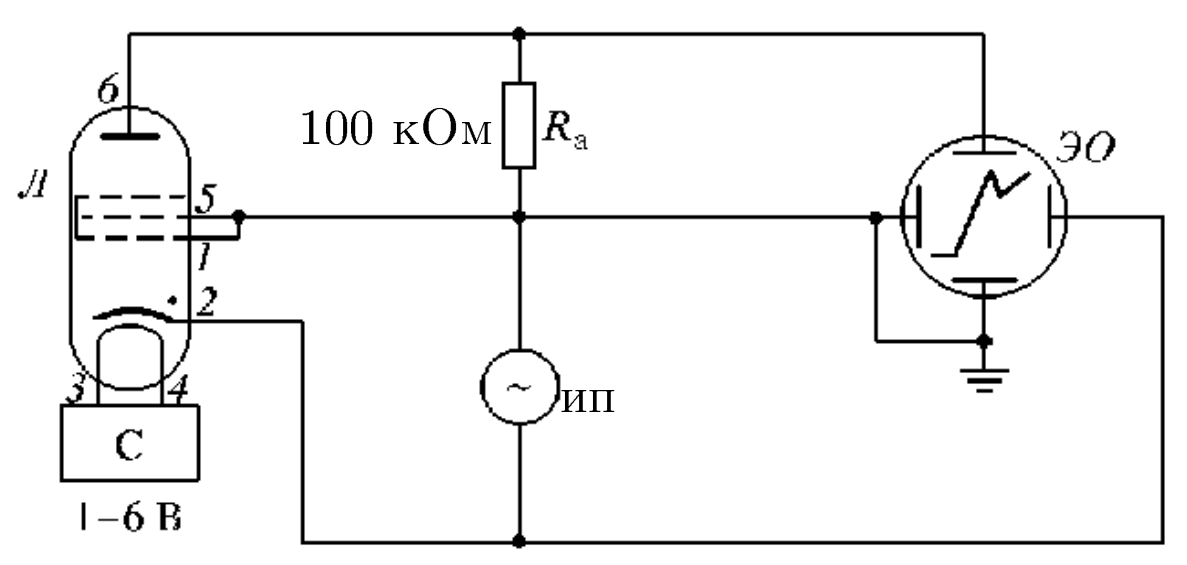
\includegraphics[width=0.3\textwidth]{img/schm1.png}
		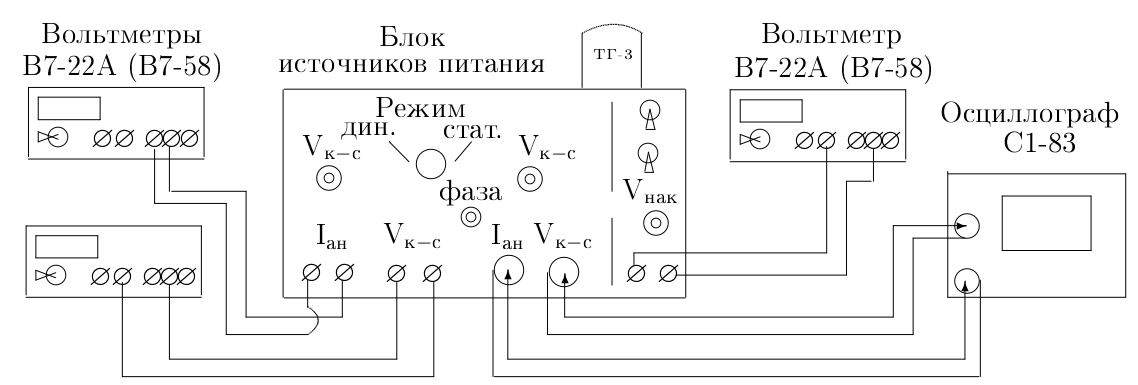
\includegraphics[width=0.6\textwidth]{img/schm2.png}
		\caption{Слева схема подключения тиратрона. Справа блок-схема экспериментальной установки.}
		\label{img:exp_scheme}
	\end{figure}

	\begin{wrapfigure}{r}{0.3\textwidth}
		\centering
		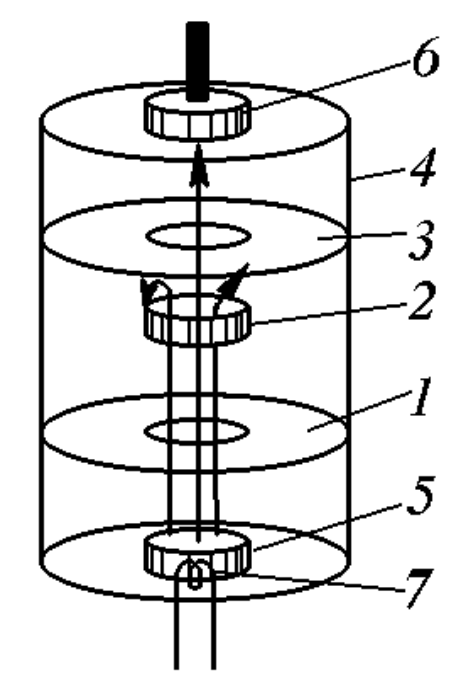
\includegraphics[width=0.15\textwidth]{img/tiratron.png}
		\caption{Схема тиратрона: 1, 2, 3 -- сетки с одинаковым потенциалом, 4 -- внешний металлический цилиндр, 5 -- катод, 6 -- анод, 7 -- накаливаемая спираль.}
		\label{img:tiratron}
	\end{wrapfigure}

	В работе для наблюдения эффекта Рамзауэра используется тиратрон ТГ3-01/1.3Б, заполненный инертным газом (рис. \ref{img:tiratron}). Электроны, эмитируемые катодом тиратрона, ускоряются напряжением $V$, приложенным между катодом и ближайшей к нему сеткой. Затем электроны рассеиваются на атомах инертного газа. Рассеянные электроны отклоняются в сторону и уходят на сетку, а оставшаяся часть электронов достигает анода и создаёт анодный ток $I_а$.
	
	Схема экспериментальной установки приведена на рисунке \ref{img:exp_scheme}. Лампа тиратрона расположена на корпусе блок источников питания. Напряжение к электродам лампы подаётся от источников питания, находящихся в корпусе прибора. Регулировка напряжения и выбор режима работы установки производится при помощи ручек управления, выведенных на лицевую панель блока источников питания.	
	
	\subsection*{Оборудование и приборы}
		
	Стенд с экспериментальной установкой номер $1.3._1$.
	\begin{enumerate}
		\item Тиратрон ТГ3-01/1.3Б.
				
		\item Вольтметры GDM-8145. Инвентарный номер вольтметра, измеряющего напряжение, пропорциональное току анода, №210104003098. Инвентарный номер вольтметра, измеряющего напряжение катод-сетка, №210104003102. Инвентарный номер вольтметра, измеряющего напряжение накала тиратрона, №210104003100. Все вольтметры измеряют в пределе 20 В. Погрешность измерения $\sigma = \pm (0.03\% \; rdg + 4 \; digits)$.
		
		\item Блок источников питания. Заводской номер №606-502. Инвентарный номер №410134125767.
		
		\item Осциллограф GOS-620. Инвентарный номер №210104000620. Коэффициент отклонения $4\%$ в диапазоне $5 \; \frac{мВ}{дел} \div 5 \; \frac{В}{дел}$.
	\end{enumerate}
	
	\subsection*{Первичные экспериментальные данные}
	
	Первичные экспериментальные данные приведены в таблице:\\
	\begin{center}
		%\DenisUpToYou
		%\input{gen/tab-data.tex}
	\end{center}

	
	
	\subsection*{Обработка экспериментальных данных}
	
	
	\subsection*{Обсуждение результатов и выводы}
	
	
\end{document}